\chapter{Исследовательская часть}

\section{Технические характеристики}

\begin{itemize}
	\item процессор -- Intel\textregistered~Core\texttrademark~i5-4590 × 4~\cite{cpu};
	\item объём оперативной памяти -- 24 ГБ;
	\item операционная система -- Ubuntu 24.04.1 LTS~\cite{ubuntu}.	
\end{itemize}

\section{Исследование}

Было проведено исследование зависимости времени генерации ландшафта от его размера. Результаты замеров приведены в таблице~\ref{tbl:mes}. График зависимости приведён на рисунке~\ref{fig:mes}.

\begin{table}[H]
	\begin{center}
		\begin{threeparttable}
			\caption{Данные замеров}
			\label{tbl:mes}
			\begin{tabular}{|c|c|}
				\hline
				n &  время генерации \\
				\hline
				2 & 94239 \\
				\hline
				3 & 100341\\
				\hline
				4 & 86143\\
				\hline 
				5 & 148750\\
				\hline 
				6 & 225966\\
				\hline
				7 & 433758\\
				\hline
				8 & 1134237\\
				\hline
				9 & 3378200\\
				\hline 
				10 & 11926117\\
				\hline
				11 & 42428064\\
				\hline
				12 & 160699571\\
				\hline
			\end{tabular}	
		\end{threeparttable}
	\end{center}
\end{table}

\begin{figure}[H]
	\centering
	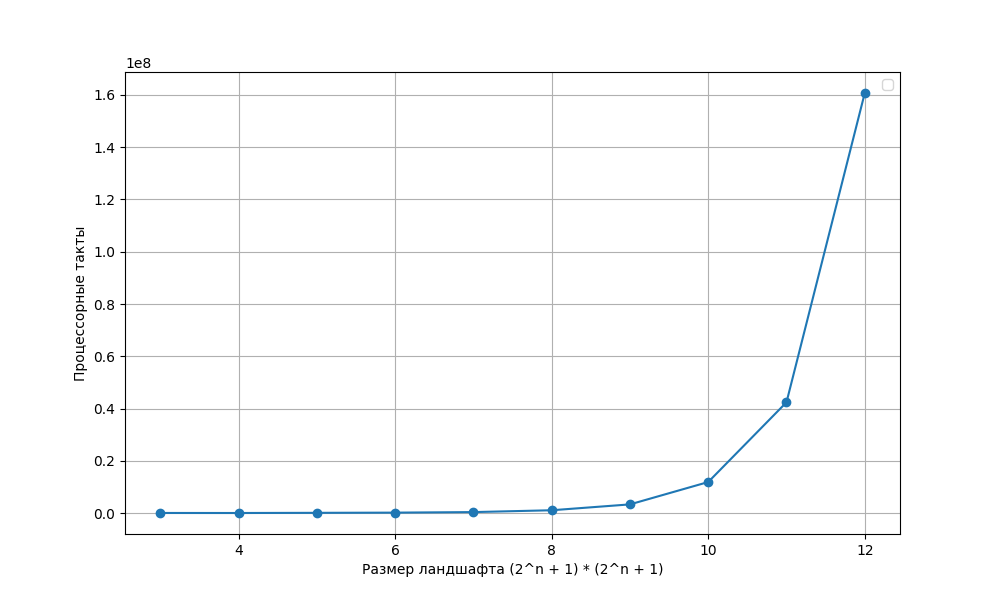
\includegraphics[height=0.4\textheight]{mes.png}
	\caption{График зависимости времени генерации ландшафта от его размера}
	\label{fig:mes}
\end{figure}

\section*{Вывод}
Из проведенного исследования можно сделать вывод: при размерах карты больших чем $(2^{11} - 1) \times (2^{11} - 1)$ алгоритм генерации ландшафта становится крайне времязатратным. 
